\documentclass[tikz, border = 5pt]{standalone}

\begin{document}
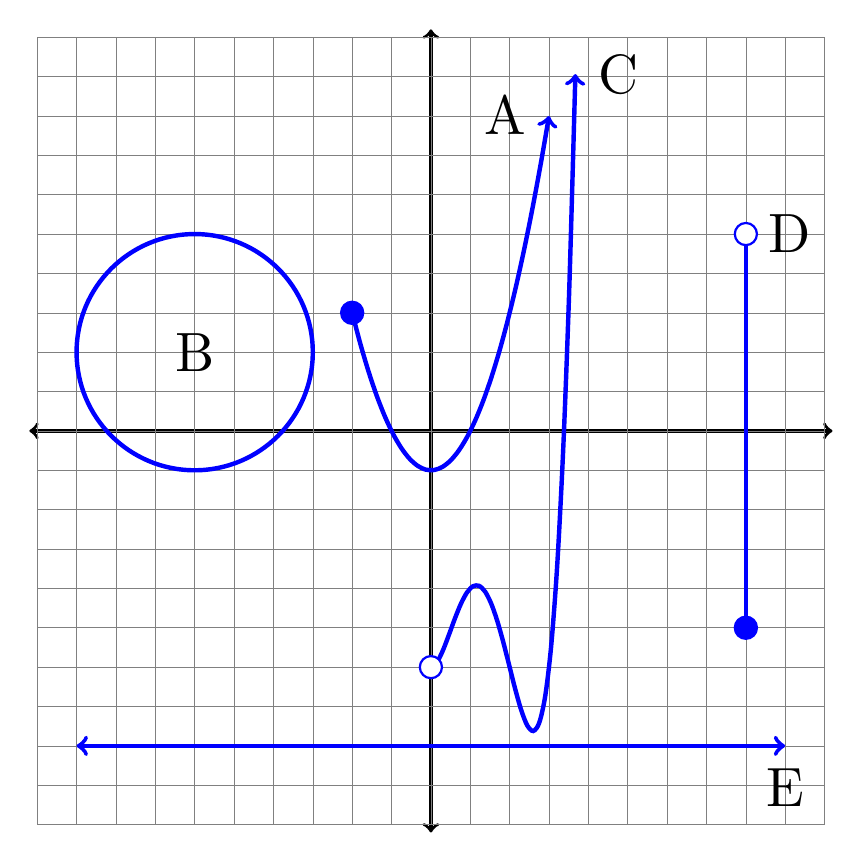
\begin{tikzpicture}
  % axis
  \draw[very thick, <->] (0, -5.1) -- (0, 5.1);
  \draw[very thick, <->] (-5.1, 0) -- (5.1, 0);

  % grid
  \draw[help lines, step = 0.5cm] (-5, -5) grid (5, 5);

\draw[ultra thick, scale=0.5, domain=-2:3,smooth,variable=\x, blue, ->] plot ({\x},{\x*\x-1}) node[left, black, scale=2] {A};
\draw [draw=blue, fill=blue, thick] (-1,1.5) circle (4.0pt);

\draw[ultra thick, blue] (-3,1) circle (1.5cm) node[black, scale=2] {B};;

\draw[ultra thick, scale=0.5, domain=0:3.67,smooth,variable=\x, blue, ->] plot ({\x},{ \x*\x*(2-\x)*(3-\x)-6 }) node[right, black, scale=2] {C};
\draw [draw=blue, fill=white, thick] (0,-3) circle (4.0pt);

\draw[ultra thick, scale=0.5, domain=-5:5,smooth,variable=\x, blue] plot ({8},{\x}) node[right, black, scale=2] {D};
\draw [draw=blue, fill=white, thick] (4,2.5) circle (4.0pt);
\draw [draw=blue, fill=blue, thick] (4,-2.5) circle (4.0pt);

\draw[ultra thick, scale=0.5, domain=-9:9,smooth,variable=\x, blue, <->] plot ({\x},{-8}) node[below, black, scale=2] {E};

\end{tikzpicture}
\end{document}
